
%% bare_jrnl.tex
%% V1.4b
%% 2015/08/26
%% by Michael Shell
%% see http://www.michaelshell.org/
%% for current contact information.
%%
%% This is a skeleton file demonstrating the use of IEEEtran.cls
%% (requires IEEEtran.cls version 1.8b or later) with an IEEE
%% journal paper.
%%
%% Support sites:
%% http://www.michaelshell.org/tex/ieeetran/
%% http://www.ctan.org/pkg/ieeetran
%% and
%% http://www.ieee.org/

%%*************************************************************************
%% Legal Notice:
%% This code is offered as-is without any warranty either expressed or
%% implied; without even the implied warranty of MERCHANTABILITY or
%% FITNESS FOR A PARTICULAR PURPOSE! 
%% User assumes all risk.
%% In no event shall the IEEE or any contributor to this code be liable for
%% any damages or losses, including, but not limited to, incidental,
%% consequential, or any other damages, resulting from the use or misuse
%% of any information contained here.
%%
%% All comments are the opinions of their respective authors and are not
%% necessarily endorsed by the IEEE.
%%
%% This work is distributed under the LaTeX Project Public License (LPPL)
%% ( http://www.latex-project.org/ ) version 1.3, and may be freely used,
%% distributed and modified. A copy of the LPPL, version 1.3, is included
%% in the base LaTeX documentation of all distributions of LaTeX released
%% 2003/12/01 or later.
%% Retain all contribution notices and credits.
%% ** Modified files should be clearly indicated as such, including  **
%% ** renaming them and changing author support contact information. **
%%*************************************************************************


% *** Authors should verify (and, if needed, correct) their LaTeX system  ***
% *** with the testflow diagnostic prior to trusting their LaTeX platform ***
% *** with production work. The IEEE's font choices and paper sizes can   ***
% *** trigger bugs that do not appear when using other class files.       ***                          ***
% The testflow support page is at:
% http://www.michaelshell.org/tex/testflow/



\documentclass[journal]{IEEEtran}

\usepackage{graphicx}
\graphicspath{ {../"Presentation & Poster"/images/} }

\usepackage{caption}
\usepackage{subcaption}

%
% If IEEEtran.cls has not been installed into the LaTeX system files,
% manually specify the path to it like:
% \documentclass[journal]{../sty/IEEEtran}





% Some very useful LaTeX packages include:
% (uncomment the ones you want to load)


% *** MISC UTILITY PACKAGES ***
%
%\usepackage{ifpdf}
% Heiko Oberdiek's ifpdf.sty is very useful if you need conditional
% compilation based on whether the output is pdf or dvi.
% usage:
% \ifpdf
%   % pdf code
% \else
%   % dvi code
% \fi
% The latest version of ifpdf.sty can be obtained from:
% http://www.ctan.org/pkg/ifpdf
% Also, note that IEEEtran.cls V1.7 and later provides a builtin
% \ifCLASSINFOpdf conditional that works the same way.
% When switching from latex to pdflatex and vice-versa, the compiler may
% have to be run twice to clear warning/error messages.






% *** CITATION PACKAGES ***
%
%\usepackage{cite}
% cite.sty was written by Donald Arseneau
% V1.6 and later of IEEEtran pre-defines the format of the cite.sty package
% \cite{} output to follow that of the IEEE. Loading the cite package will
% result in citation numbers being automatically sorted and properly
% "compressed/ranged". e.g., [1], [9], [2], [7], [5], [6] without using
% cite.sty will become [1], [2], [5]--[7], [9] using cite.sty. cite.sty's
% \cite will automatically add leading space, if needed. Use cite.sty's
% noadjust option (cite.sty V3.8 and later) if you want to turn this off
% such as if a citation ever needs to be enclosed in parenthesis.
% cite.sty is already installed on most LaTeX systems. Be sure and use
% version 5.0 (2009-03-20) and later if using hyperref.sty.
% The latest version can be obtained at:
% http://www.ctan.org/pkg/cite
% The documentation is contained in the cite.sty file itself.






% *** GRAPHICS RELATED PACKAGES ***
%
\ifCLASSINFOpdf
  % \usepackage[pdftex]{graphicx}
  % declare the path(s) where your graphic files are
  % \graphicspath{{../pdf/}{../jpeg/}}
  % and their extensions so you won't have to specify these with
  % every instance of \includegraphics
  % \DeclareGraphicsExtensions{.pdf,.jpeg,.png}
\else
  % or other class option (dvipsone, dvipdf, if not using dvips). graphicx
  % will default to the driver specified in the system graphics.cfg if no
  % driver is specified.
  % \usepackage[dvips]{graphicx}
  % declare the path(s) where your graphic files are
  % \graphicspath{{../eps/}}
  % and their extensions so you won't have to specify these with
  % every instance of \includegraphics
  % \DeclareGraphicsExtensions{.eps}
\fi
% graphicx was written by David Carlisle and Sebastian Rahtz. It is
% required if you want graphics, photos, etc. graphicx.sty is already
% installed on most LaTeX systems. The latest version and documentation
% can be obtained at: 
% http://www.ctan.org/pkg/graphicx
% Another good source of documentation is "Using Imported Graphics in
% LaTeX2e" by Keith Reckdahl which can be found at:
% http://www.ctan.org/pkg/epslatex
%
% latex, and pdflatex in dvi mode, support graphics in encapsulated
% postscript (.eps) format. pdflatex in pdf mode supports graphics
% in .pdf, .jpeg, .png and .mps (metapost) formats. Users should ensure
% that all non-photo figures use a vector format (.eps, .pdf, .mps) and
% not a bitmapped formats (.jpeg, .png). The IEEE frowns on bitmapped formats
% which can result in "jaggedy"/blurry rendering of lines and letters as
% well as large increases in file sizes.
%
% You can find documentation about the pdfTeX application at:
% http://www.tug.org/applications/pdftex





% *** MATH PACKAGES ***
%
%\usepackage{amsmath}
% A popular package from the American Mathematical Society that provides
% many useful and powerful commands for dealing with mathematics.
%
% Note that the amsmath package sets \interdisplaylinepenalty to 10000
% thus preventing page breaks from occurring within multiline equations. Use:
%\interdisplaylinepenalty=2500
% after loading amsmath to restore such page breaks as IEEEtran.cls normally
% does. amsmath.sty is already installed on most LaTeX systems. The latest
% version and documentation can be obtained at:
% http://www.ctan.org/pkg/amsmath





% *** SPECIALIZED LIST PACKAGES ***
%
%\usepackage{algorithmic}
% algorithmic.sty was written by Peter Williams and Rogerio Brito.
% This package provides an algorithmic environment fo describing algorithms.
% You can use the algorithmic environment in-text or within a figure
% environment to provide for a floating algorithm. Do NOT use the algorithm
% floating environment provided by algorithm.sty (by the same authors) or
% algorithm2e.sty (by Christophe Fiorio) as the IEEE does not use dedicated
% algorithm float types and packages that provide these will not provide
% correct IEEE style captions. The latest version and documentation of
% algorithmic.sty can be obtained at:
% http://www.ctan.org/pkg/algorithms
% Also of interest may be the (relatively newer and more customizable)
% algorithmicx.sty package by Szasz Janos:
% http://www.ctan.org/pkg/algorithmicx




% *** ALIGNMENT PACKAGES ***
%
%\usepackage{array}
% Frank Mittelbach's and David Carlisle's array.sty patches and improves
% the standard LaTeX2e array and tabular environments to provide better
% appearance and additional user controls. As the default LaTeX2e table
% generation code is lacking to the point of almost being broken with
% respect to the quality of the end results, all users are strongly
% advised to use an enhanced (at the very least that provided by array.sty)
% set of table tools. array.sty is already installed on most systems. The
% latest version and documentation can be obtained at:
% http://www.ctan.org/pkg/array


% IEEEtran contains the IEEEeqnarray family of commands that can be used to
% generate multiline equations as well as matrices, tables, etc., of high
% quality.




% *** SUBFIGURE PACKAGES ***
%\ifCLASSOPTIONcompsoc
%  \usepackage[caption=false,font=normalsize,labelfont=sf,textfont=sf]{subfig}
%\else
%  \usepackage[caption=false,font=footnotesize]{subfig}
%\fi
% subfig.sty, written by Steven Douglas Cochran, is the modern replacement
% for subfigure.sty, the latter of which is no longer maintained and is
% incompatible with some LaTeX packages including fixltx2e. However,
% subfig.sty requires and automatically loads Axel Sommerfeldt's caption.sty
% which will override IEEEtran.cls' handling of captions and this will result
% in non-IEEE style figure/table captions. To prevent this problem, be sure
% and invoke subfig.sty's "caption=false" package option (available since
% subfig.sty version 1.3, 2005/06/28) as this is will preserve IEEEtran.cls
% handling of captions.
% Note that the Computer Society format requires a larger sans serif font
% than the serif footnote size font used in traditional IEEE formatting
% and thus the need to invoke different subfig.sty package options depending
% on whether compsoc mode has been enabled.
%
% The latest version and documentation of subfig.sty can be obtained at:
% http://www.ctan.org/pkg/subfig




% *** FLOAT PACKAGES ***
%
%\usepackage{fixltx2e}
% fixltx2e, the successor to the earlier fix2col.sty, was written by
% Frank Mittelbach and David Carlisle. This package corrects a few problems
% in the LaTeX2e kernel, the most notable of which is that in current
% LaTeX2e releases, the ordering of single and double column floats is not
% guaranteed to be preserved. Thus, an unpatched LaTeX2e can allow a
% single column figure to be placed prior to an earlier double column
% figure.
% Be aware that LaTeX2e kernels dated 2015 and later have fixltx2e.sty's
% corrections already built into the system in which case a warning will
% be issued if an attempt is made to load fixltx2e.sty as it is no longer
% needed.
% The latest version and documentation can be found at:
% http://www.ctan.org/pkg/fixltx2e


%\usepackage{stfloats}
% stfloats.sty was written by Sigitas Tolusis. This package gives LaTeX2e
% the ability to do double column floats at the bottom of the page as well
% as the top. (e.g., "\begin{figure*}[!b]" is not normally possible in
% LaTeX2e). It also provides a command:
%\fnbelowfloat
% to enable the placement of footnotes below bottom floats (the standard
% LaTeX2e kernel puts them above bottom floats). This is an invasive package
% which rewrites many portions of the LaTeX2e float routines. It may not work
% with other packages that modify the LaTeX2e float routines. The latest
% version and documentation can be obtained at:
% http://www.ctan.org/pkg/stfloats
% Do not use the stfloats baselinefloat ability as the IEEE does not allow
% \baselineskip to stretch. Authors submitting work to the IEEE should note
% that the IEEE rarely uses double column equations and that authors should try
% to avoid such use. Do not be tempted to use the cuted.sty or midfloat.sty
% packages (also by Sigitas Tolusis) as the IEEE does not format its papers in
% such ways.
% Do not attempt to use stfloats with fixltx2e as they are incompatible.
% Instead, use Morten Hogholm'a dblfloatfix which combines the features
% of both fixltx2e and stfloats:
%
% \usepackage{dblfloatfix}
% The latest version can be found at:
% http://www.ctan.org/pkg/dblfloatfix




%\ifCLASSOPTIONcaptionsoff
%  \usepackage[nomarkers]{endfloat}
% \let\MYoriglatexcaption\caption
% \renewcommand{\caption}[2][\relax]{\MYoriglatexcaption[#2]{#2}}
%\fi
% endfloat.sty was written by James Darrell McCauley, Jeff Goldberg and 
% Axel Sommerfeldt. This package may be useful when used in conjunction with 
% IEEEtran.cls'  captionsoff option. Some IEEE journals/societies require that
% submissions have lists of figures/tables at the end of the paper and that
% figures/tables without any captions are placed on a page by themselves at
% the end of the document. If needed, the draftcls IEEEtran class option or
% \CLASSINPUTbaselinestretch interface can be used to increase the line
% spacing as well. Be sure and use the nomarkers option of endfloat to
% prevent endfloat from "marking" where the figures would have been placed
% in the text. The two hack lines of code above are a slight modification of
% that suggested by in the endfloat docs (section 8.4.1) to ensure that
% the full captions always appear in the list of figures/tables - even if
% the user used the short optional argument of \caption[]{}.
% IEEE papers do not typically make use of \caption[]'s optional argument,
% so this should not be an issue. A similar trick can be used to disable
% captions of packages such as subfig.sty that lack options to turn off
% the subcaptions:
% For subfig.sty:
% \let\MYorigsubfloat\subfloat
% \renewcommand{\subfloat}[2][\relax]{\MYorigsubfloat[]{#2}}
% However, the above trick will not work if both optional arguments of
% the \subfloat command are used. Furthermore, there needs to be a
% description of each subfigure *somewhere* and endfloat does not add
% subfigure captions to its list of figures. Thus, the best approach is to
% avoid the use of subfigure captions (many IEEE journals avoid them anyway)
% and instead reference/explain all the subfigures within the main caption.
% The latest version of endfloat.sty and its documentation can obtained at:
% http://www.ctan.org/pkg/endfloat
%
% The IEEEtran \ifCLASSOPTIONcaptionsoff conditional can also be used
% later in the document, say, to conditionally put the References on a 
% page by themselves.




% *** PDF, URL AND HYPERLINK PACKAGES ***
%
%\usepackage{url}
% url.sty was written by Donald Arseneau. It provides better support for
% handling and breaking URLs. url.sty is already installed on most LaTeX
% systems. The latest version and documentation can be obtained at:
% http://www.ctan.org/pkg/url
% Basically, \url{my_url_here}.




% *** Do not adjust lengths that control margins, column widths, etc. ***
% *** Do not use packages that alter fonts (such as pslatex).         ***
% There should be no need to do such things with IEEEtran.cls V1.6 and later.
% (Unless specifically asked to do so by the journal or conference you plan
% to submit to, of course. )


% correct bad hyphenation here
\hyphenation{op-tical net-works semi-conduc-tor}


\begin{document}
%
% paper title
% Titles are generally capitalized except for words such as a, an, and, as,
% at, but, by, for, in, nor, of, on, or, the, to and up, which are usually
% not capitalized unless they are the first or last word of the title.
% Linebreaks \\ can be used within to get better formatting as desired.
% Do not put math or special symbols in the title.
\title{Dice Pip Detection}
%
%
% author names and IEEE memberships
% note positions of commas and nonbreaking spaces ( ~ ) LaTeX will not break
% a structure at a ~ so this keeps an author's name from being broken across
% two lines.
% use \thanks{} to gain access to the first footnote area
% a separate \thanks must be used for each paragraph as LaTeX2e's \thanks
% was not built to handle multiple paragraphs
%

\author{James Young}

% note the % following the last \IEEEmembership and also \thanks - 
% these prevent an unwanted space from occurring between the last author name
% and the end of the author line. i.e., if you had this:
% 
% \author{....lastname \thanks{...} \thanks{...} }
%                     ^------------^------------^----Do not want these spaces!
%
% a space would be appended to the last name and could cause every name on that
% line to be shifted left slightly. This is one of those "LaTeX things". For
% instance, "\textbf{A} \textbf{B}" will typeset as "A B" not "AB". To get
% "AB" then you have to do: "\textbf{A}\textbf{B}"
% \thanks is no different in this regard, so shield the last } of each \thanks
% that ends a line with a % and do not let a space in before the next \thanks.
% Spaces after \IEEEmembership other than the last one are OK (and needed) as
% you are supposed to have spaces between the names. For what it is worth,
% this is a minor point as most people would not even notice if the said evil
% space somehow managed to creep in.



% The paper headers
\markboth{CS 504: Machine Vision - Final Project}%
{Shell \MakeLowercase{\textit{et al.}}: Bare Demo of IEEEtran.cls for IEEE Journals}
% The only time the second header will appear is for the odd numbered pages
% after the title page when using the twoside option.
% 
% *** Note that you probably will NOT want to include the author's ***
% *** name in the headers of peer review papers.                   ***
% You can use \ifCLASSOPTIONpeerreview for conditional compilation here if
% you desire.




% If you want to put a publisher's ID mark on the page you can do it like
% this:
%\IEEEpubid{0000--0000/00\$00.00~\copyright~2015 IEEE}
% Remember, if you use this you must call \IEEEpubidadjcol in the second
% column for its text to clear the IEEEpubid mark.



% use for special paper notices
%\IEEEspecialpapernotice{(Invited Paper)}




% make the title area
\maketitle

% As a general rule, do not put math, special symbols or citations
% in the abstract or keywords.
\begin{abstract}
Inspired by table-top games, this project aimed to develop a program that would provide a meaningful application of machine vision techniques learned in this semester. The program itself takes an input image of rolled dice, and outputs where dice are located, as well the number of pips on the upwards face. In its current state, the program is capable of detecting 89.13\% of rolled dice, with 100\% accuracy in counting the pips of detected dice. Beyond this point, the program has many avenues of continuation, such as integration into actual applications, to improving the underlying code.
\end{abstract}

% Note that keywords are not normally used for peerreview papers.
\begin{IEEEkeywords}
machine vision, dice detection, table-top games
\end{IEEEkeywords}

% For peer review papers, you can put extra information on the cover
% page as needed:
% \ifCLASSOPTIONpeerreview
% \begin{center} \bfseries EDICS Category: 3-BBND \end{center}
% \fi
%
% For peerreview papers, this IEEEtran command inserts a page break and
% creates the second title. It will be ignored for other modes.
\IEEEpeerreviewmaketitle



\section{Introduction}
% The very first letter is a 2 line initial drop letter followed
% by the rest of the first word in caps.
% 
% form to use if the first word consists of a single letter:
% \IEEEPARstart{A}{demo} file is ....
% 
% form to use if you need the single drop letter followed by
% normal text (unknown if ever used by the IEEE):
% \IEEEPARstart{A}{}demo file is ....
% 
% Some journals put the first two words in caps:
% \IEEEPARstart{T}{his demo} file is ....
% 
% Here we have the typical use of a "T" for an initial drop letter
% and "HIS" in caps to complete the first word.
\IEEEPARstart{T}{his} project was first thought of as both a fun and challenging application of machine vision as well as an extension to another program I have been developing for the past year.\\

To give some background, I greatly enjoy table-top gaming as a hobby and have regularly played with a group for years. However, since progressing into graduate school, as well as the majority of the group also going their own ways, we no longer had an easy way to continue playing. Not one to give up, a solution proposed was to develop a chat client bot that would facilitate many of the physical aspects of table-top gaming; the first and foremost being dice rolling. This application became known as GoblinBot (affectionately named from the fantasy creature found in some of the more well known table-top games).\\

The primary purpose of GoblinBot is to provide the ability to roll dice in a manner such that all players can see the result easily. Thankfully, having this based as a chat client bot, all results are returned via a message from the bot. This solved the most practical problem of playing these games over the internet, but some issues still remained. One element that makes these games exciting is making critical rolls (no pun intended) and watching the dice settle- for better or for worse. Even with GoblinBot, there is a loss of this anticipation or excitement, as at the end of the day, the bot is still just an electronic program.\\

This is where this program comes into the picture; a melding between the analog and digital. In the lens of GoblinBot, longer standing goal of this project is to eventually tie it into the already existing program with hopes that it provides an improvement to the overall experience. Outside of this, this project seemed like a reasonable challenge to undertake. Having completed the work, it certainly was and I believe that it was a good summation of much of what was taught in the Machine Vision course.\\



% An example of a floating figure using the graphicx package.
% Note that \label must occur AFTER (or within) \caption.
% For figures, \caption should occur after the \includegraphics.
% Note that IEEEtran v1.7 and later has special internal code that
% is designed to preserve the operation of \label within \caption
% even when the captionsoff option is in effect. However, because
% of issues like this, it may be the safest practice to put all your
% \label just after \caption rather than within \caption{}.
%
% Reminder: the "draftcls" or "draftclsnofoot", not "draft", class
% option should be used if it is desired that the figures are to be
% displayed while in draft mode.
%
%\begin{figure}[!t]
%\centering
%\includegraphics[width=2.5in]{myfigure}
% where an .eps filename suffix will be assumed under latex, 
% and a .pdf suffix will be assumed for pdflatex; or what has been declared
% via \DeclareGraphicsExtensions.
%\caption{Simulation results for the network.}
%\label{fig_sim}
%\end{figure}

% Note that the IEEE typically puts floats only at the top, even when this
% results in a large percentage of a column being occupied by floats.


% An example of a double column floating figure using two subfigures.
% (The subfig.sty package must be loaded for this to work.)
% The subfigure \label commands are set within each subfloat command,
% and the \label for the overall figure must come after \caption.
% \hfil is used as a separator to get equal spacing.
% Watch out that the combined width of all the subfigures on a 
% line do not exceed the text width or a line break will occur.
%
%\begin{figure*}[!t]
%\centering
%\subfloat[Case I]{\includegraphics[width=2.5in]{box}%
%\label{fig_first_case}}
%\hfil
%\subfloat[Case II]{\includegraphics[width=2.5in]{box}%
%\label{fig_second_case}}
%\caption{Simulation results for the network.}
%\label{fig_sim}
%\end{figure*}
%
% Note that often IEEE papers with subfigures do not employ subfigure
% captions (using the optional argument to \subfloat[]), but instead will
% reference/describe all of them (a), (b), etc., within the main caption.
% Be aware that for subfig.sty to generate the (a), (b), etc., subfigure
% labels, the optional argument to \subfloat must be present. If a
% subcaption is not desired, just leave its contents blank,
% e.g., \subfloat[].


% An example of a floating table. Note that, for IEEE style tables, the
% \caption command should come BEFORE the table and, given that table
% captions serve much like titles, are usually capitalized except for words
% such as a, an, and, as, at, but, by, for, in, nor, of, on, or, the, to
% and up, which are usually not capitalized unless they are the first or
% last word of the caption. Table text will default to \footnotesize as
% the IEEE normally uses this smaller font for tables.
% The \label must come after \caption as always.
%
%\begin{table}[!t]
%% increase table row spacing, adjust to taste
%\renewcommand{\arraystretch}{1.3}
% if using array.sty, it might be a good idea to tweak the value of
% \extrarowheight as needed to properly center the text within the cells
%\caption{An Example of a Table}
%\label{table_example}
%\centering
%% Some packages, such as MDW tools, offer better commands for making tables
%% than the plain LaTeX2e tabular which is used here.
%\begin{tabular}{|c||c|}
%\hline
%One & Two\\
%\hline
%Three & Four\\
%\hline
%\end{tabular}
%\end{table}


% Note that the IEEE does not put floats in the very first column
% - or typically anywhere on the first page for that matter. Also,
% in-text middle ("here") positioning is typically not used, but it
% is allowed and encouraged for Computer Society conferences (but
% not Computer Society journals). Most IEEE journals/conferences use
% top floats exclusively. 
% Note that, LaTeX2e, unlike IEEE journals/conferences, places
% footnotes above bottom floats. This can be corrected via the
% \fnbelowfloat command of the stfloats package.


\section{Project Goals}
This project had two major goals to achieve in order to produce an ideal program.
\begin{itemize}
	\item Be able to detect dice and count the pips.
	\item Be able to do detection within a reasonable frame rate.
\end{itemize}

\section{Program Overview/Approach}
The main problem needed to be solved by this program is to be able to take in an input image, and through a series of transformations/thresholds/etc. be able to isolate both the dice as well as it's pips. Every step of note in this process will be discussed such that it can be easily understood and re-implemented.

\subsection{Grab Input}
To begin the detection process, the program needs a background image (no dice present) (Fig. \ref{fig:background_input}) from which it can use to differentiate from the foreground image (dice present) (Fig. \ref{fig:foreground_input}).

\begin{figure}[h]
	
\includegraphics[width=8cm]{BG}
	\centering
	\caption{The background supplied}
	\label{fig:background_input}
\end{figure}
\begin{figure}[h]
	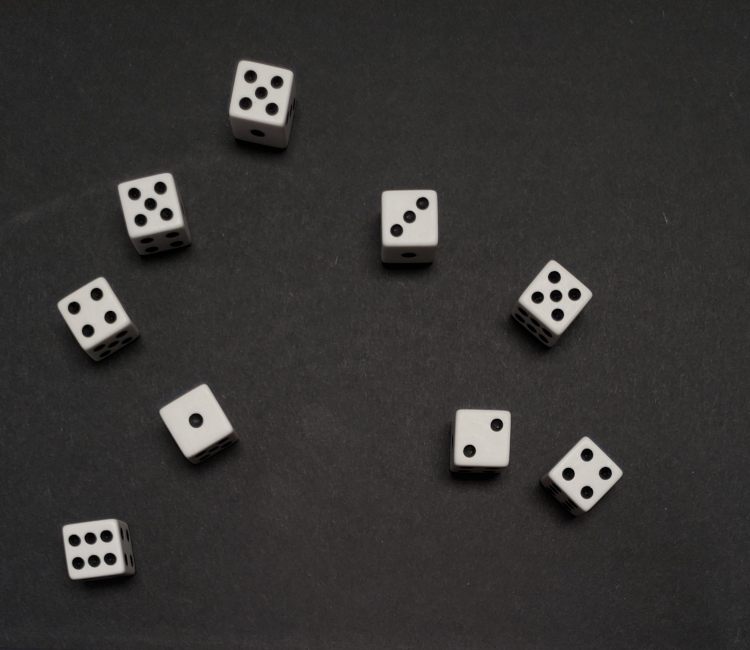
\includegraphics[width=8cm]{FG}
	\centering
	\caption{The foreground supplied}
	\label{fig:foreground_input}
\end{figure}

\subsection{Obtain Difference}
Once the foreground and background images have been read in, then a difference between the two images is performed (Fig. \ref{fig:fgbg_difference}). This begins the process of finding the regions of interest where the dice are located.\\

\begin{figure}[h]
	\includegraphics[width=8cm]{"FGBG Difference"}
	\centering
	\caption{Difference between background and foreground}
	\label{fig:fgbg_difference}
\end{figure}


\subsection{Gaussian Blur and Otsu's Threshold}
Gaussian Blur and Otsu's Threshold (Fig. \ref{fig:otsu_threshold}) is applied to the image to prepare it for Canny Edge detection.\\
\begin{figure}[h]
	\includegraphics[width=8cm]{"Otsu1"}
	\centering
	\caption{Otsu's Threshold}
	\label{fig:otsu_threshold}
\end{figure}

\subsection{Canny Edge Detection}
Canny Edge detection is performed (Fig. \ref{fig:canny_edges}), and at this point the actual dice detection begins.\\
\begin{figure}[h]
	\includegraphics[width=8cm]{"CannyEdges"}
	\centering
	\caption{Canny Edge Detection}
	\label{fig:canny_edges}
\end{figure}

\subsection{Find and Iterate Through Contours}
With the Canny Edge detection performed, the program begins to look at all of the closed contours found in the image. If the closed contour found is larger than a specified size (to avoid grabbing singular pips, along other small noise), it will then pass that contour onto a sub-process which will extract and count the pips.\\

\subsubsection{Use Contour to Obtain Bounding Box}
Once a contour of sufficient size has been found, a bounding box is calculated.\\

\subsubsection{Crop Out Sub-Image}
Using the calculated bounding box, the region is then cropped out of the original foreground image. By cropping from the original input image, it provides the ability to look at more detail on each individual dice by using more specialized parameters.\\

\subsubsection{Resize}
With the isolated and cropped out dice, the image is then resized to amplify details and ease the detection of pips (Fig. \ref{fig:small_crop}). In this case, the size was doubled.\\

\begin{figure}[h]
	\includegraphics[width=4cm]{"small_crop"}
	\centering
	\caption{Cropped and Enlarged Die}
	\label{fig:small_crop}
\end{figure}

\subsubsection{Gaussian Blur}
Like in earlier steps, Gaussian blur is applied to improve performance of subsequent operations (Fig. \ref{fig:small_blur}).\\

\begin{figure}[h]
	\includegraphics[width=4cm]{"small_blur"}
	\centering
	\caption{Gaussian Blur Applied}
	\label{fig:small_blur}
\end{figure}

\subsubsection{Otsu's Threshold}
Application of Otsu's Threshold to further bring out pips from the surrounding dice face (Fig. \ref{fig:small_otsu}).\\

\begin{figure}[h]
	\includegraphics[width=4cm]{"small_otsu"}
	\centering
	\caption{Otsu's Threshold Applied}
	\label{fig:small_otsu}
\end{figure}

\subsubsection{Bucket Fill Corners}
At this point, blob detection can be performed, but the application of bucket filling the corners ensures that the pips, and only the pips, are left when blob detection is run. As the name implies, the program takes the four corners of the image and fills with white pixels (Fig. \ref{fig:small_bucketfill}).\\

\begin{figure}[h]
	\includegraphics[width=4cm]{"small_bucketfill"}
	\centering
	\caption{Bucket Fill Corners}
	\label{fig:small_bucketfill}
\end{figure}

\subsubsection{Use Blob Detection to Count Pips}
Finally, with the pips being completely isolated, blob detection is used, and the number of detected blobs is counted, giving the number of pips on the die (Fig. \ref{fig:small_blob}).\\

\begin{figure}[h]
	\includegraphics[width=4cm]{"small_blob"}
	\centering
	\caption{Count Pips via Blob Detection}
	\label{fig:small_blob}
\end{figure}

\subsection{Draw Bounding Boxes and Pip Count}
After running on each closed contour, the program then draws each bounding box and corresponding number of pips, resulting in the final output (Fig. \ref{fig:final_output_red}).\\

\begin{figure}[h]
	\includegraphics[width=8cm]{"Final_output_red"}
	\centering
	\caption{Final Output with Bounding Boxes and Number of Pips Drawn}
	\label{fig:final_output_red}
\end{figure}

\section{Results}
The immediate results of this project show that the program can detect 89.13\% of dice, with a 100\% accuracy rate when counting the pips on detected dice. It should be noted however that these results were taken from a small set of five test images, four of which consisted of rolled dice, and one being manually set up. In addition, two additional images were provided containing edge case scenarios: Immediately Adjacent Dice and Overlapping Dice. The program was unable to detect dice in these two images.\\

Performance-wise, frame rate was investigated by looping the operations and recording how long it took to process each loop. When testing this, frame rate never dropped below 5 frames per second, even with a great deal of debug code running in tandem.\\



\begin{figure}
	\centering
	\begin{subfigure}{.25\textwidth}
		\centering
		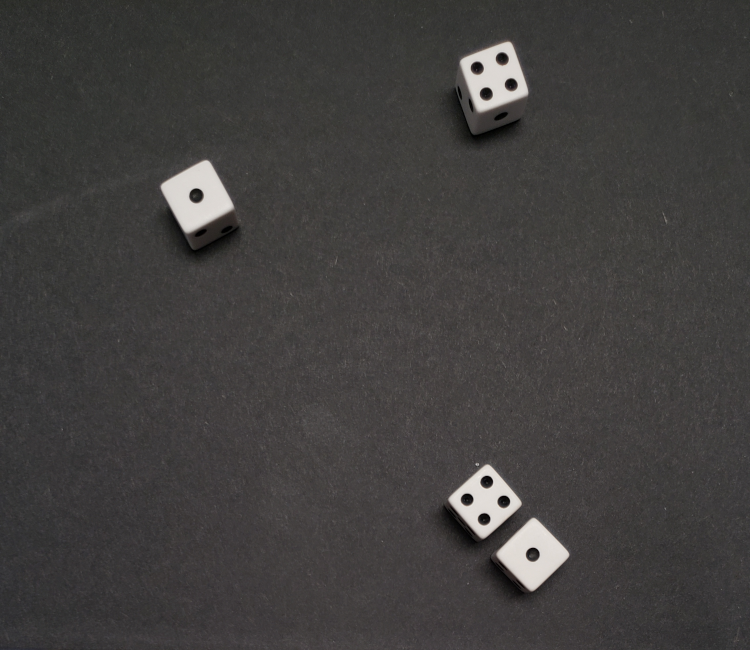
\includegraphics[width=.95\linewidth]{image1}
		\caption{Input}
		\label{fig:results1_sub1}
	\end{subfigure}%
	\begin{subfigure}{.25\textwidth}
		\centering
		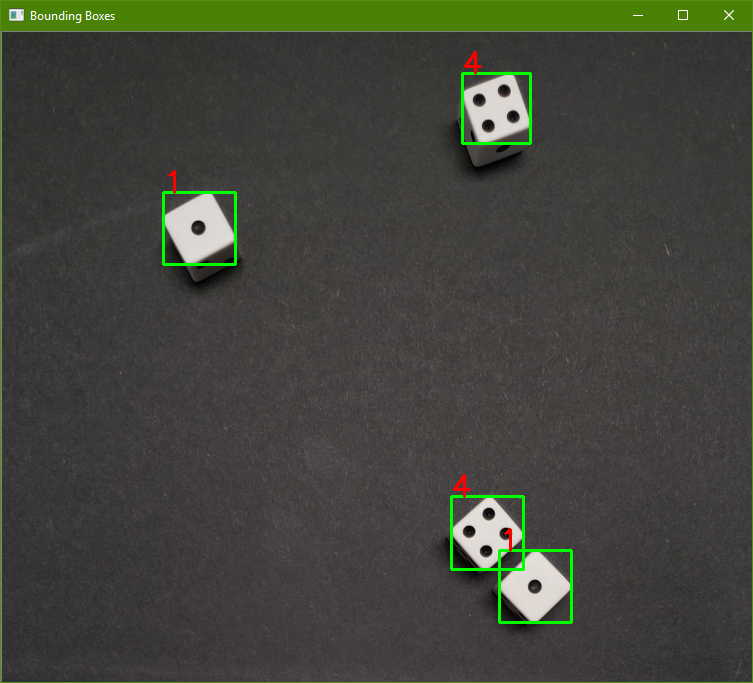
\includegraphics[width=.95\linewidth]{image1_output}
		\caption{Output}
		\label{fig:results1_sub2}
	\end{subfigure}
	\caption{Input and Output using test image 1}
	\label{fig:results1}
\end{figure}


\begin{figure}
	\centering
	\begin{subfigure}{.25\textwidth}
		\centering
		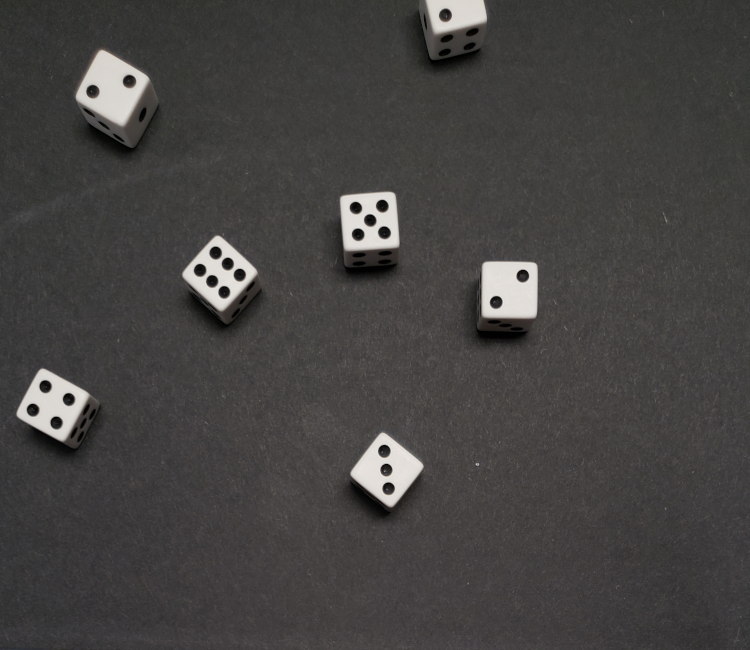
\includegraphics[width=.95\linewidth]{image2}
		\caption{Input}
		\label{fig:results2_sub1}
	\end{subfigure}%
	\begin{subfigure}{.25\textwidth}
		\centering
		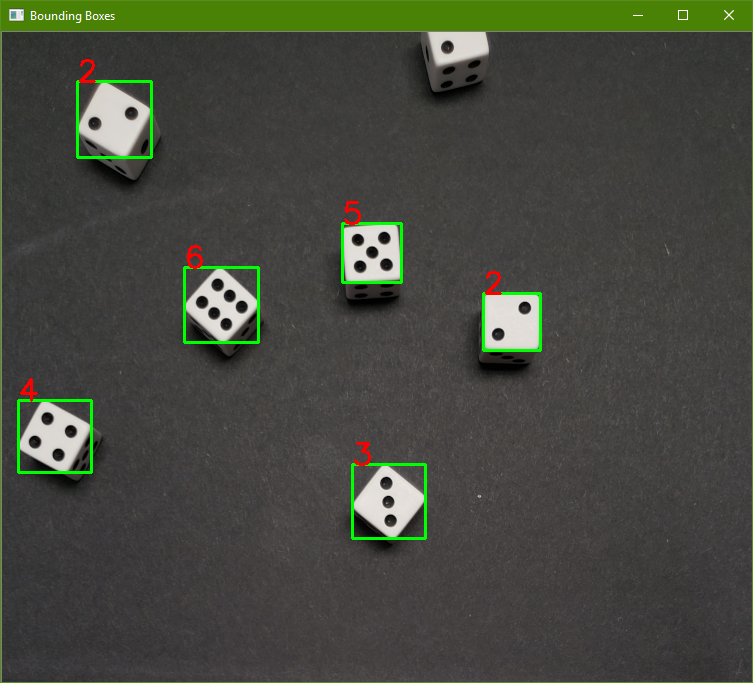
\includegraphics[width=.95\linewidth]{image2_output}
		\caption{Output}
		\label{fig:results2_sub2}
	\end{subfigure}
	\caption{Input and Output using test image 2}
	\label{fig:results2}
\end{figure}


\begin{figure}
	\centering
	\begin{subfigure}{.25\textwidth}
		\centering
		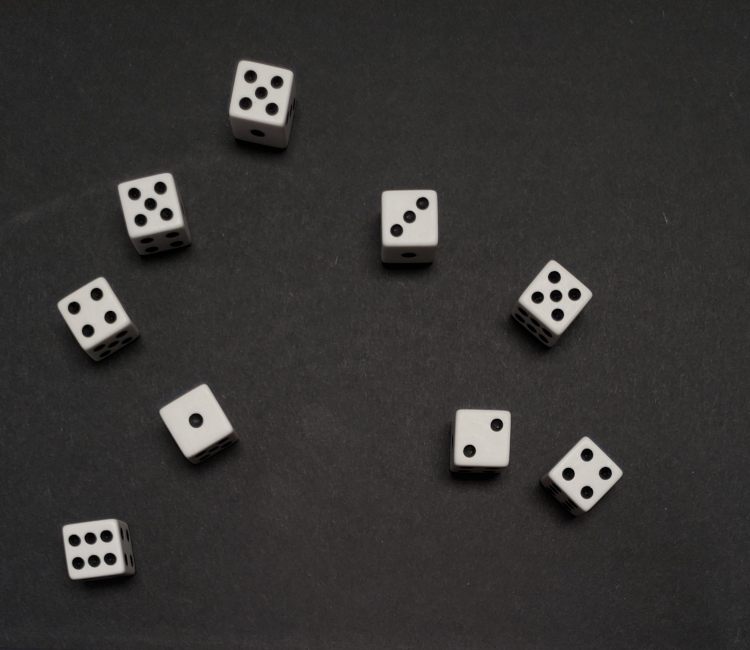
\includegraphics[width=.95\linewidth]{image3}
		\caption{Input}
		\label{fig:results3_sub1}
	\end{subfigure}%
	\begin{subfigure}{.25\textwidth}
		\centering
		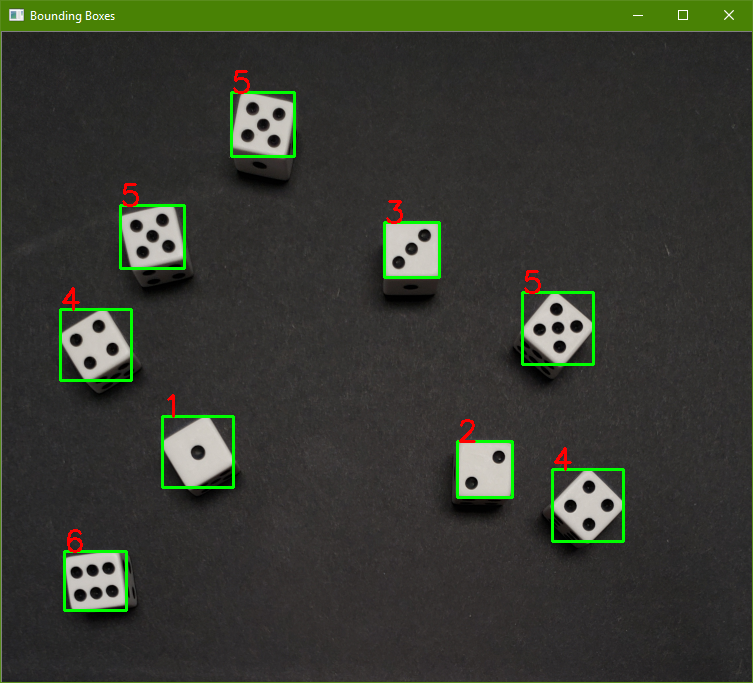
\includegraphics[width=.95\linewidth]{image3_output}
		\caption{Output}
		\label{fig:results3_sub2}
	\end{subfigure}
	\caption{Input and Output using test image 3}
	\label{fig:results3}
\end{figure}


\begin{figure}
	\centering
	\begin{subfigure}{.25\textwidth}
		\centering
		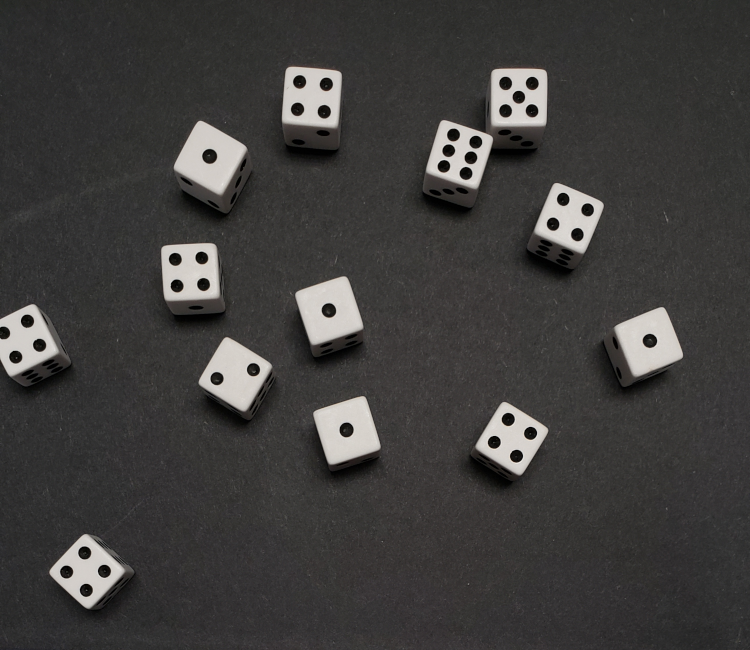
\includegraphics[width=.95\linewidth]{image4}
		\caption{Input}
		\label{fig:results4_sub1}
	\end{subfigure}%
	\begin{subfigure}{.25\textwidth}
		\centering
		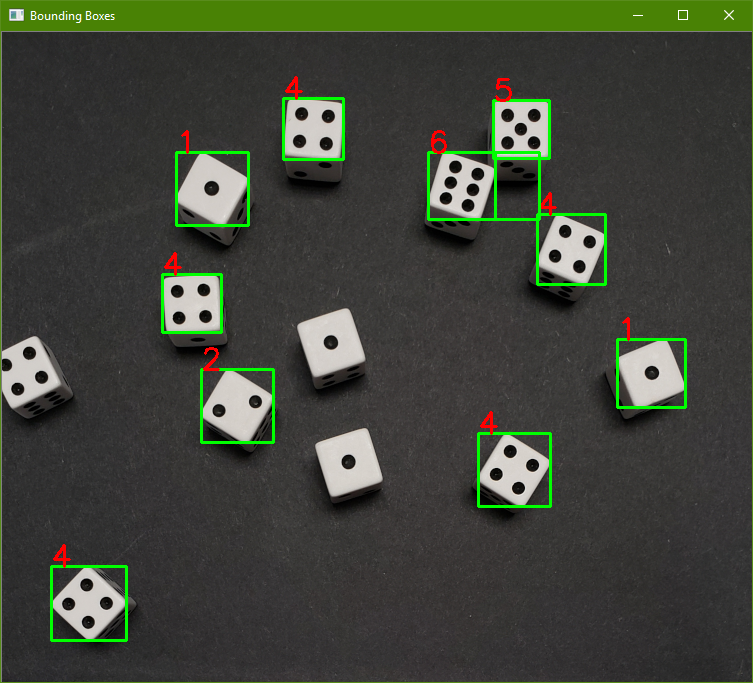
\includegraphics[width=.95\linewidth]{image4_output}
		\caption{Output}
		\label{fig:results4_sub2}
	\end{subfigure}
	\caption{Input and Output using test image 4}
	\label{fig:results4}
\end{figure}

\begin{figure}
	\centering
	\begin{subfigure}{.25\textwidth}
		\centering
		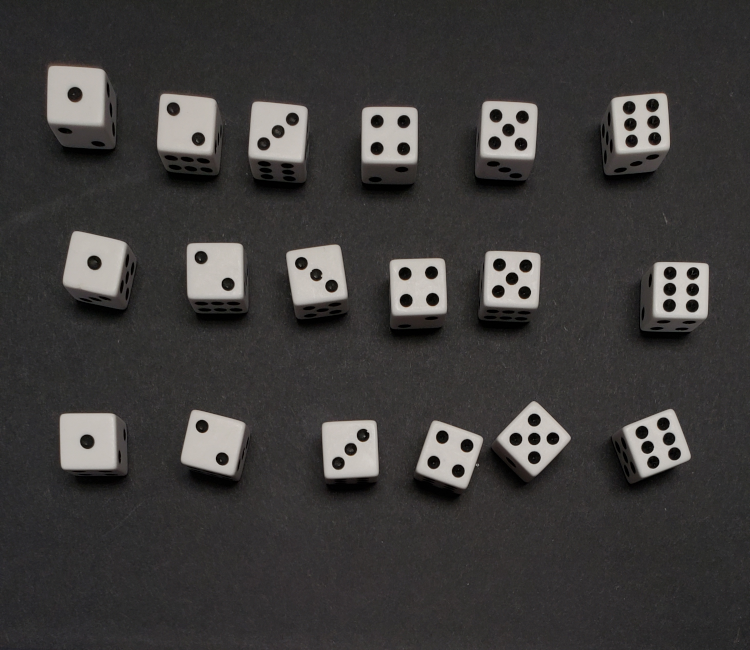
\includegraphics[width=.95\linewidth]{image5}
		\caption{Input}
		\label{fig:results5_sub1}
	\end{subfigure}%
	\begin{subfigure}{.25\textwidth}
		\centering
		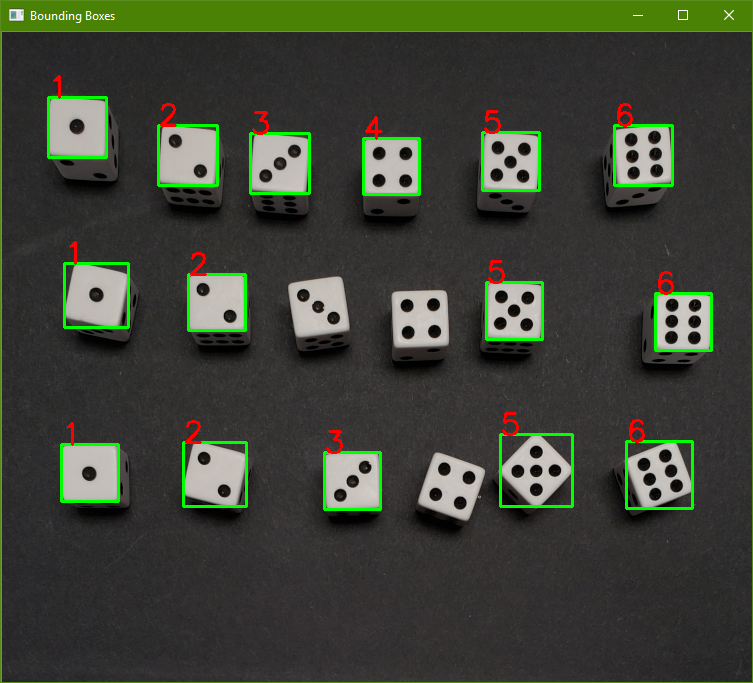
\includegraphics[width=.95\linewidth]{image5_output}
		\caption{Output}
		\label{fig:results5_sub2}
	\end{subfigure}
	\caption{Input and Output using test image 5}
	\label{fig:results5}
\end{figure}

\begin{figure}
	\centering
	\begin{subfigure}{.25\textwidth}
		\centering
		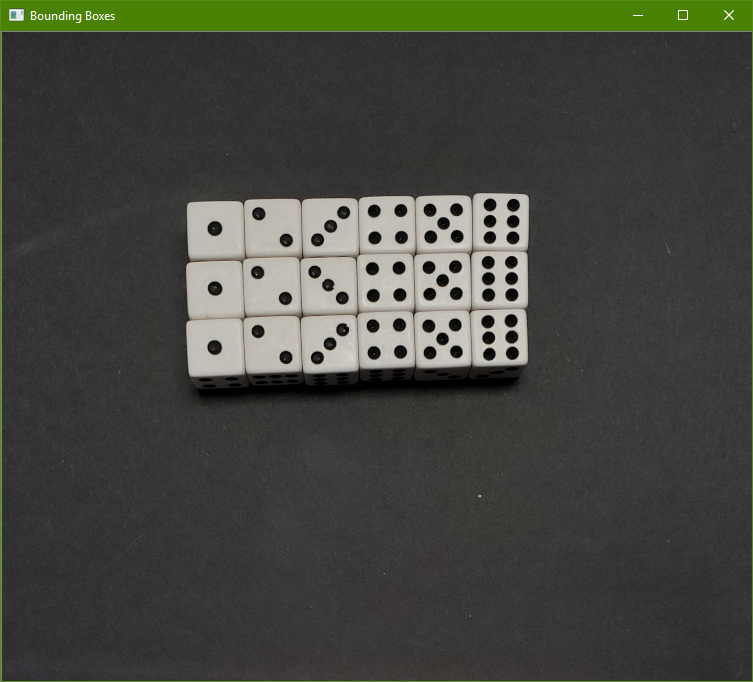
\includegraphics[width=.95\linewidth]{adjacent_1}
		\caption{Input}
		\label{fig:adjacent_sub1}
	\end{subfigure}%
	\begin{subfigure}{.25\textwidth}
		\centering
		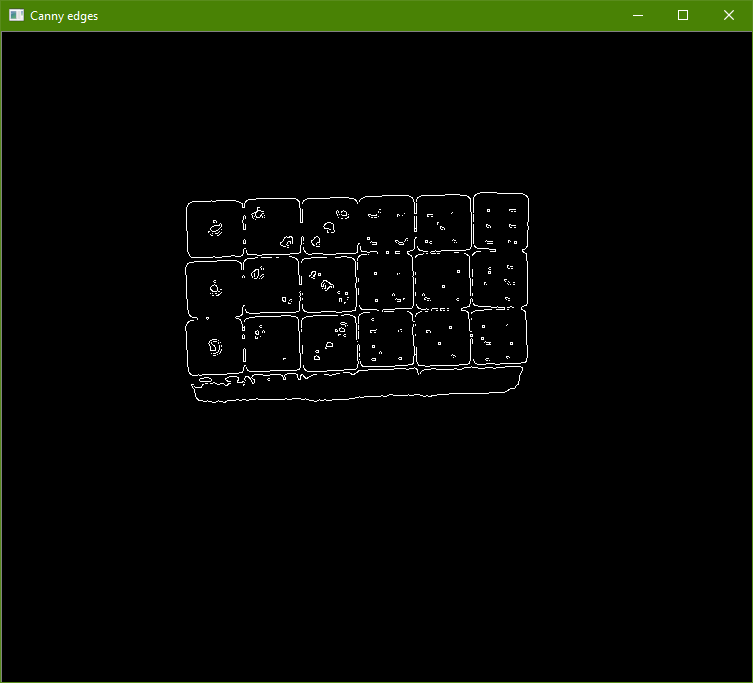
\includegraphics[width=.95\linewidth]{adjacent_2}
		\caption{Canny Edge Detection}
		\label{fig:adjacent_sub2}
	\end{subfigure}
	\caption{Input and Canny Edge using test image 6 (edge case)}
	\label{fig:adjancet}
\end{figure}

\begin{figure}
	\centering
	\begin{subfigure}{.25\textwidth}
		\centering
		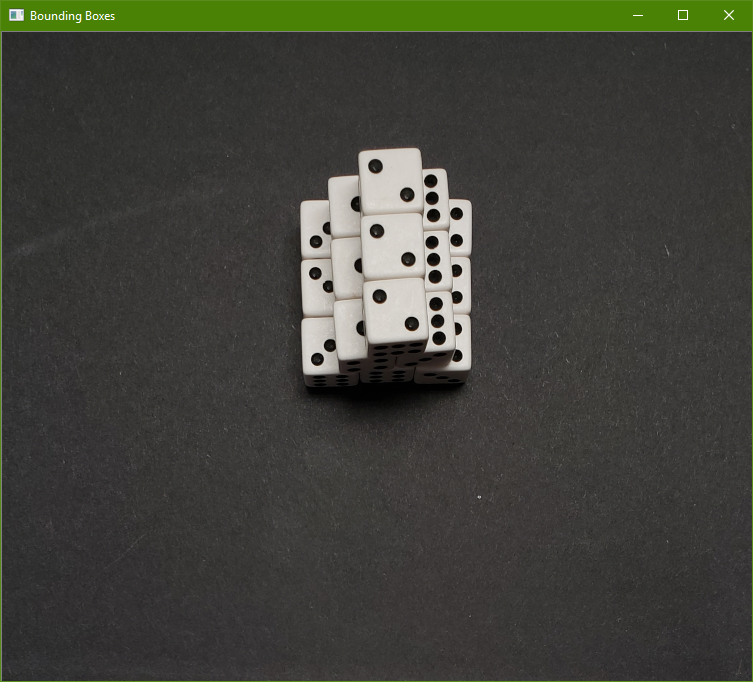
\includegraphics[width=.95\linewidth]{overlapping_1}
		\caption{Input}
		\label{fig:overlapping_sub1}
	\end{subfigure}%
	\begin{subfigure}{.25\textwidth}
		\centering
		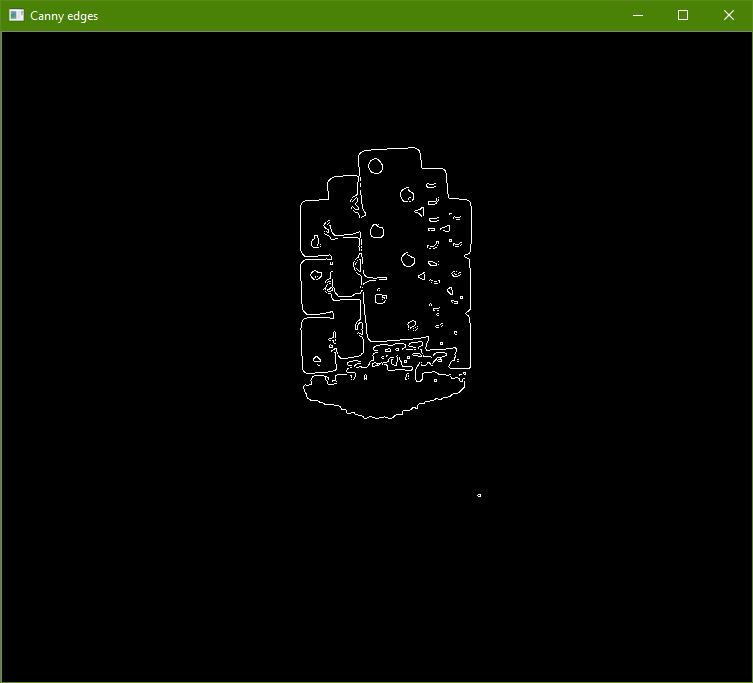
\includegraphics[width=.95\linewidth]{overlapping_2}
		\caption{Canny Edge Detection}
		\label{fig:overlapping_sub2}
	\end{subfigure}
	\caption{Input and Canny Edge using test image 7 (edge case)}
	\label{fig:overlapping}
\end{figure}

\begin{figure}[h]
	\includegraphics[width=8cm]{"pixel_gaps_2"}
	\centering
	\caption{Canny Edge detection from test image 5}
	\label{fig:pixel_gaps_canny}
\end{figure}

\begin{figure}
	\centering
	\begin{subfigure}{.25\textwidth}
		\centering
		
\includegraphics[width=.95\linewidth]{pixel_gap1}
		\caption{Fourth Dice, Last Row}
		\label{fig:pixel_gaps_sub1}
	\end{subfigure}%
	\begin{subfigure}{.25\textwidth}
		\centering
		
\includegraphics[width=.95\linewidth]{pixel_gap2}
		\caption{Third Dice, Middle Row}
		\label{fig:pixel_gaps_sub2}
	\end{subfigure}
	\caption{Zoomed in image of un-closed contours from test image 5}
	\label{fig:pixel_gaps}
\end{figure}



\section{Discussion}
Having started work on this program from scratch, these results are quite exciting. Drawing from figures \ref{fig:results1} to \ref{fig:results5} we can see many different, interesting aspects. As mentioned earlier, the first four test images were of actual dice rolls, with the fifth being a more controlled setup to better gauge the performance of multiple dice.\\

In figure \ref{fig:results1}, we can see that the four dice were all correctly located and counted, with two dice in the lower right being relatively close. While maybe not as interesting as what follows, this shows a good baseline application/use case of the program\\

In figure \ref{fig:results2}, things start to get a little more interesting. All dice that were rolled within frame were able to be located and counted, leaving out the die out of frame. When looking over the results of this image, it was quite encouraging that the program did not miscount the dice as only having one pip, and instead ignoring it. This exclusion is primarily due to the contour not being closed, which could be an issue should the closed contours no longer be a criteria for detection. For the time being however, it does its job and produces ideal results.\\

Figure \ref{fig:results3} is the best result produced by the program, in that it is able to get 100\% detection, 100\% accuracy on counting, as well as being rolled naturally. Not much else needs to be said about this figure, other than that this is the ideal performance for the program.\\

Figure \ref{fig:results4} starts to show some of the issues in the dice detection. First, the two dice in the center, showing ones, are not picked up by the program. Second, the bounding box on the six in the upper right is heavily stretched out in comparison to the intended box shape. Since the non-detection problem is so large, discussion of that will be in a later section, and for now the focus will be on the misshapen bounding box. To the best of my understanding, this is a result of the program picking up the side of five dice right next to it, thus increasing the size of the box. Thankfully, likely due to the lighting, the pips on the side of the die are not counted, and it still gets the correct value of six.\\

Finally, figure \ref{fig:results5} shows the similar issues of non-detection. This being the case, the program is still able to detect the large majority of dice in the image, as well as correctly counting the pips.\\

Moving onto the topic of non-detection, figure \ref{fig:pixel_gaps_canny} shows the Canny Edge detection from test image 5, and figure \ref{fig:pixel_gaps} (a) and (b) show a zoomed in version of a couple of the non-detected dice. As described earlier, the program checks for closed contours to consider the region to be of interest or not, and as can be seen here, there are small gaps in the contours. While the program is fairly robust in avoiding noise (mostly due to the heavy constraints used to handle the input) it cannot fully avoid it even in more controlled environments, and certainly not in other environments. The take-away from this is that this would be one of the next steps in developing this program- figuring out a solution to close, or circumvent, the gaps in contours.\\

Currently, the biggest issue this program faces is its inability to detect 100\% of the dice in the image. Unfortunately, given the time frame of this project I was unable to fix these issues in time, however below are some of the potential solutions to this problem.

\begin{itemize}
	\item Use better parameters to improve each step involved in the edge detection/contouring process.
	\item Use morphology to attempt to patch the small gaps.
	\item Suggested in the presentation portion of this project, use the fact that the dice face is square to allow for a more flexible detection scheme (so long as the contour is mostly a square, it should be able to detect)
	
\end{itemize}


Beyond the initial set of test images, two additional images were taken and used as input for the program. The goal with these two edge case images were to see if any insight could be gained from how the program handled the images, as well as to sate simple curiosity. In figures \ref{fig:adjancet} (adjacent dice) and \ref{fig:overlapping} (overlapping dice), the input image, as well as its Canny Edge detection are shown. The biggest take away from these sets of images is to see how the contour is shaped, which by extension explains why the detection failed. While it is fairly clear that the overlapping input would have a great deal of trouble reaching a state where it could be successfully detected, the adjacent input is quite close to forming closed contours. Detection could likely be achieved by additional fine-tuning of the various parameters.\\

Finally, as far as the frame rate is concerned, I believe it reaches the goal of being reasonable. The frame rate was never a problem during the development phase, and if it was, there is still a great deal of room for optimization.\\



\section{Conclusion}
As far as I am concerned, this project can be seen as a success. While the goal of detection was not achieved 100\%, the ground work to reach that point is absolutely present. The project itself was quite enjoyable to work on as well, which is always a plus. Beyond that, the following two subsections discuss directions that this work could go in, both internally and externally.\\


\subsection{Future Work}
This section describes potential extensions of the work done in this project.\\

\subsubsection{Improve Detection/Bug Fixes}
The immediate steps to be taken with this project would be to fix the errors with the dice detection, namely fixing the issue of small gaps in the contours. Beyond this, there are small improvements to parameters and other aspects that could be undertaken as well, such as removing the constraint of requiring a background image for detection, or modifying the program that it is more flexible in what it considers a valid contour that denotes a die.\\

\subsubsection{Broaden Detection Scope}
Beyond direct improvements to the program, another area of future work would be to achieve colored dice and numbered dice detection. Initially, this project was to detect colored dice due to their widespread use, but this was constrained due to the additional difficulty it posed when trying to detect them. While the program currently only covered dice with pips, another extension of this project would be to detect dice with numbers on them. The proposed approach to this problem is to isolate the dice in a much, if not completely, similar way, but then use more advanced methods than blob detection to read the number from the die face. One such method might be to use a machine learning model, trained on detecting numbers to read the value.\\

\subsubsection{Machine Learning Approach}
While this is slightly covered in the previous section, this would be a machine learning implementation of the whole process. One of the larger problems with this however is the lack of a good data set, but with a good enough data set, this approach would presumably be much more flexible. Some of the major gains would be the loosening of the heavy constraints placed on how the input images have to be taken, as well as being able to easily train the model on both pips and numbers.\\
\subsection{Applications}
While similar to future work in the sense that this would be what would naturally following the completion of this project, this section will focus more on the external aspects of how this program can be taken and used, rather than internal improvements.\\

\subsubsection{Augmented Reality Dice Games}
Probably the easiest to work with, one application of this program would be to apply it to simple dice games such as Yahtzee or Farkle. Since the program is able to read in many different aspects of rolled dice and then use them in a digital manner, a natural progression would be to use this as input to a game. While it would depend on the game, the only elements that would need to be added is game states/turns, as well as keeping score. Beyond this, additional flair and aspects can be programmed in to produce a more interesting and exciting display.\\

\subsubsection{Phone Application or Tool}
Closer to the original goal/inspiration for this project, this program could also be used as a tool to assist table-top gaming. In the most general case, the ability to quickly count, as well as potentially sum, a large amount of dice is invaluable given many complex table-top games. Rolling up to eight dice at a time is often common, and there are situations in some games that require up to rolling as many as forty dice, all at once, to perform an action. Being able to speed up the process of counting dice would almost certainly translate into faster games.\\

\subsubsection{Bringing Physical Aspects to Network Play}
Closest now to the inspiration of the project is the idea of bringing aspects of in-person play to an online session. One of the larger issues for playing traditionally table-top games over the internet is the inherent lack of having all players in one spot. One of the biggest appeal to table-top gaming is being able to have face-to-face interaction with the other players, which is wholly removed when playing over the internet. This application of the program in this way would be doing no more than providing some helpful tools to otherwise a webcam focused on some dice, but the intent is that it adds the sense of physicality to an otherwise wholly virtual game session.\\


% if have a single appendix:
%\appendix[Proof of the Zonklar Equations]
% or
%\appendix  % for no appendix heading
% do not use \section anymore after \appendix, only \section*
% is possibly needed

% use appendices with more than one appendix
% then use \section to start each appendix
% you must declare a \section before using any
% \subsection or using \label (\appendices by itself
% starts a section numbered zero.)
%



% Can use something like this to put references on a page
% by themselves when using endfloat and the captionsoff option.


% trigger a \newpage just before the given reference
% number - used to balance the columns on the last page
% adjust value as needed - may need to be readjusted if
% the document is modified later
%\IEEEtriggeratref{8}
% The "triggered" command can be changed if desired:
%\IEEEtriggercmd{\enlargethispage{-5in}}

% references section

% can use a bibliography generated by BibTeX as a .bbl file
% BibTeX documentation can be easily obtained at:
% http://mirror.ctan.org/biblio/bibtex/contrib/doc/
% The IEEEtran BibTeX style support page is at:
% http://www.michaelshell.org/tex/ieeetran/bibtex/
%\bibliographystyle{IEEEtran}
% argument is your BibTeX string definitions and bibliography database(s)
%\bibliography{IEEEabrv,../bib/paper}
%
% <OR> manually copy in the resultant .bbl file
% set second argument of \begin to the number of references
% (used to reserve space for the reference number labels box)

% biography section
% 
% If you have an EPS/PDF photo (graphicx package needed) extra braces are
% needed around the contents of the optional argument to biography to prevent
% the LaTeX parser from getting confused when it sees the complicated
% \includegraphics command within an optional argument. (You could create
% your own custom macro containing the \includegraphics command to make things
% simpler here.)
%\begin{IEEEbiography}[{\includegraphics[width=1in,height=1.25in,clip,keepaspectratio]{mshell}}]{Michael Shell}
% or if you just want to reserve a space for a photo:

% if you will not have a photo at all:


% insert where needed to balance the two columns on the last page with
% biographies
%\newpage


% You can push biographies down or up by placing
% a \vfill before or after them. The appropriate
% use of \vfill depends on what kind of text is
% on the last page and whether or not the columns
% are being equalized.

%\vfill

% Can be used to pull up biographies so that the bottom of the last one
% is flush with the other column.
%\enlargethispage{-5in}



% that's all folks
\end{document}


